\documentclass[9pt,twocolumn,twoside,]{pnas-new}

%% Some pieces required from the pandoc template
\providecommand{\tightlist}{%
  \setlength{\itemsep}{0pt}\setlength{\parskip}{0pt}}

% Use the lineno option to display guide line numbers if required.
% Note that the use of elements such as single-column equations
% may affect the guide line number alignment.


\usepackage[T1]{fontenc}
\usepackage[utf8]{inputenc}

% For Pandoc highlighting needs
\usepackage{color}
\usepackage{fancyvrb}
\newcommand{\VerbBar}{|}
\newcommand{\VERB}{\Verb[commandchars=\\\{\}]}
\DefineVerbatimEnvironment{Highlighting}{Verbatim}{commandchars=\\\{\}}
% Add ',fontsize=\small' for more characters per line
\newenvironment{Shaded}{}{}
\newcommand{\AlertTok}[1]{\textcolor[rgb]{1.00,0.00,0.00}{\textbf{#1}}}
\newcommand{\AnnotationTok}[1]{\textcolor[rgb]{0.38,0.63,0.69}{\textbf{\textit{#1}}}}
\newcommand{\AttributeTok}[1]{\textcolor[rgb]{0.49,0.56,0.16}{#1}}
\newcommand{\BaseNTok}[1]{\textcolor[rgb]{0.25,0.63,0.44}{#1}}
\newcommand{\BuiltInTok}[1]{#1}
\newcommand{\CharTok}[1]{\textcolor[rgb]{0.25,0.44,0.63}{#1}}
\newcommand{\CommentTok}[1]{\textcolor[rgb]{0.38,0.63,0.69}{\textit{#1}}}
\newcommand{\CommentVarTok}[1]{\textcolor[rgb]{0.38,0.63,0.69}{\textbf{\textit{#1}}}}
\newcommand{\ConstantTok}[1]{\textcolor[rgb]{0.53,0.00,0.00}{#1}}
\newcommand{\ControlFlowTok}[1]{\textcolor[rgb]{0.00,0.44,0.13}{\textbf{#1}}}
\newcommand{\DataTypeTok}[1]{\textcolor[rgb]{0.56,0.13,0.00}{#1}}
\newcommand{\DecValTok}[1]{\textcolor[rgb]{0.25,0.63,0.44}{#1}}
\newcommand{\DocumentationTok}[1]{\textcolor[rgb]{0.73,0.13,0.13}{\textit{#1}}}
\newcommand{\ErrorTok}[1]{\textcolor[rgb]{1.00,0.00,0.00}{\textbf{#1}}}
\newcommand{\ExtensionTok}[1]{#1}
\newcommand{\FloatTok}[1]{\textcolor[rgb]{0.25,0.63,0.44}{#1}}
\newcommand{\FunctionTok}[1]{\textcolor[rgb]{0.02,0.16,0.49}{#1}}
\newcommand{\ImportTok}[1]{#1}
\newcommand{\InformationTok}[1]{\textcolor[rgb]{0.38,0.63,0.69}{\textbf{\textit{#1}}}}
\newcommand{\KeywordTok}[1]{\textcolor[rgb]{0.00,0.44,0.13}{\textbf{#1}}}
\newcommand{\NormalTok}[1]{#1}
\newcommand{\OperatorTok}[1]{\textcolor[rgb]{0.40,0.40,0.40}{#1}}
\newcommand{\OtherTok}[1]{\textcolor[rgb]{0.00,0.44,0.13}{#1}}
\newcommand{\PreprocessorTok}[1]{\textcolor[rgb]{0.74,0.48,0.00}{#1}}
\newcommand{\RegionMarkerTok}[1]{#1}
\newcommand{\SpecialCharTok}[1]{\textcolor[rgb]{0.25,0.44,0.63}{#1}}
\newcommand{\SpecialStringTok}[1]{\textcolor[rgb]{0.73,0.40,0.53}{#1}}
\newcommand{\StringTok}[1]{\textcolor[rgb]{0.25,0.44,0.63}{#1}}
\newcommand{\VariableTok}[1]{\textcolor[rgb]{0.10,0.09,0.49}{#1}}
\newcommand{\VerbatimStringTok}[1]{\textcolor[rgb]{0.25,0.44,0.63}{#1}}
\newcommand{\WarningTok}[1]{\textcolor[rgb]{0.38,0.63,0.69}{\textbf{\textit{#1}}}}

% Pandoc citation processing
\newlength{\csllabelwidth}
\setlength{\csllabelwidth}{3em}
\newlength{\cslhangindent}
\setlength{\cslhangindent}{1.5em}
% for Pandoc 2.8 to 2.10.1
\newenvironment{cslreferences}%
  {}%
  {\par}
% For Pandoc 2.11+
\newenvironment{CSLReferences}[2] % #1 hanging-ident, #2 entry spacing
 {% don't indent paragraphs
  \setlength{\parindent}{0pt}
  % turn on hanging indent if param 1 is 1
  \ifodd #1 \everypar{\setlength{\hangindent}{\cslhangindent}}\ignorespaces\fi
  % set entry spacing
  \ifnum #2 > 0
  \setlength{\parskip}{#2\baselineskip}
  \fi
 }%
 {}
\usepackage{calc} % for calculating minipage widths
\newcommand{\CSLBlock}[1]{#1\hfill\break}
\newcommand{\CSLLeftMargin}[1]{\parbox[t]{\csllabelwidth}{#1}}
\newcommand{\CSLRightInline}[1]{\parbox[t]{\linewidth - \csllabelwidth}{#1}\break}
\newcommand{\CSLIndent}[1]{\hspace{\cslhangindent}#1}


\templatetype{pnasresearcharticle}  % Choose template

\title{Estimación de parámetros de la distribución de meses de
supervivencia libre de cáncer colorrectal}

\author[a,1,2]{Carlos Lezama}
\author[a,1,2]{Marco Medina}
\author[a,1,2]{Emiliano Ramírez}
\author[a,1,2]{Santiago Villarreal}

  \affil[a]{Instituto Tecnológico Autónomo de México}


% Please give the surname of the lead author for the running footer
\leadauthor{Lezama, Medina, Ramírez y Villarreal}

% Please add here a significance statement to explain the relevance of your work
\significancestatement{}


\authorcontributions{}


\equalauthors{\textsuperscript{1} Todos los autores contribuyeron a este
trabajo por igual.}

\correspondingauthor{\textsuperscript{2} Trabajo presentado para el
curso de \textbf{Simulación (EST-24107)} impartido por Jorge Francisco
de la Vega Góngora. E-mail:
\href{mailto:jorge.delavegagongora@gmail.com}{\nolinkurl{jorge.delavegagongora@gmail.com}}}

% Keywords are not mandatory, but authors are strongly encouraged to provide them. If provided, please include two to five keywords, separated by the pipe symbol, e.g:
 \keywords{  aproximación estocástica |  ćancer
colorrectal |  estimación |  optimización numérica  } 

\begin{abstract}
En el presente proyecto se estiman los parámetros de una distribución
gamma para los datos de meses antes de recaer en casos de cáncer de
colon. El algoritmo aplicado usa técnicas de optimización numérica,
simulación y estadística para aproximar los híper-parámetros de la
distribución. Para la solución del problema, nos basamos en el trabajo
de Andrew Gelman.
\end{abstract}

\dates{This manuscript was compiled on \today}
\doi{\url{www.pnas.org/cgi/doi/10.1073/pnas.XXXXXXXXXX}}

\begin{document}

% Optional adjustment to line up main text (after abstract) of first page with line numbers, when using both lineno and twocolumn options.
% You should only change this length when you've finalised the article contents.
\verticaladjustment{-2pt}

\maketitle
\thispagestyle{firststyle}
\ifthenelse{\boolean{shortarticle}}{\ifthenelse{\boolean{singlecolumn}}{\abscontentformatted}{\abscontent}}{}

% If your first paragraph (i.e. with the \dropcap) contains a list environment (quote, quotation, theorem, definition, enumerate, itemize...), the line after the list may have some extra indentation. If this is the case, add \parshape=0 to the end of the list environment.

\acknow{}

\hypertarget{introducciuxf3n}{%
\section*{Introducción}\label{introducciuxf3n}}
\addcontentsline{toc}{section}{Introducción}

De acuerdo a la Organización Mundial de la Salud, una de cada seis
muertes en el mundo se debe al cáncer, conviertiéndole en la segunda
causa de muerte a nivel global. En 2018, el cáncer fue responsable de
aproximadamente 9.6 millones de muertes a nivel global. La mayoría de
las muertes por cáncer están asociadas con malos hábitos: mala
alimentación, falta de actividad física, así como el uso y abuso de
sustancias como el tabaco y el alcohol. En la mayoría de los países, el
cáncer se ubica como uno de los principales problemas de salud pública,
sobre todo en aquellos países de ingreso medio o bajo.

En México, de acuerdo a la Agencia Internacional para la Investigación
en Cáncer de la OMS, estima que el cáncer de colon y recto es el tercero
más frecuente en México, con 14,900 casos nuevos por año. Las cifras de
esta enfermedad parecen seguir en aumento, y una de las principales
razones está relacionada con la falta de conocimiento de este cáncer por
parte del sistema de salud, particularmente en conocer la distribución
de su reaparición meses después de concluir tratamientos oncológicos.

Estudiar la distribución de los meses que transcurren antes de una
reaparición de cáncer es de especial importancia ya que ayudará a
entender mejor la efectividad de los tratamientos contra el cáncer e
incluso brindaría información acerca de la persistencia del tipo de
cáncer ya se por condiciones genéticas o patológicas del individuo.

En este proyecto, exploramos un método para estimar la distribución del
número de meses libres de cáncer colorrectal antes de su reaparición,
mediante un método de momentos utilizando simulaciones Monte Carlo. El
problema consiste en estimar desde un enfoque de Optimización los
parámetros de la distribución a priori que se supone siguen los datos.
En este caso, dada la característica de supervivencia que tienen los
datos de meses antes de la reparación de cáncer (donde podemos
interpretar al evento ``cáncer colorrectal reaparece'' como el evento
exitoso) suponemos que la distribución sigue una distribución
\(Gamma(\alpha, \beta)\).

Ahora bien, la estimación por método de momentos con estimaciones Monte
Carlo y Newton-Raphson tiene una utilidad especial ya que es efectivo
cuando los momentos de la distribución y sus derivadas no tienen forma
analítica cerrada ya sea por construcción de la función o porque
simplemente no se conoce. Es decir, dados los datos de la realización de
alguna variable aleatoria puedes imponer condiciones a la distribución,
en términos de momentos y parámetros, para adjudicarle alguna propiedad
de interés que la literatura diga sobre tu conjunto de datos y estimar
dichos momentos con este método. El alcance pragmático del método es
amplio para este tipo de problemas pues es una herramienta que se puede
usar cuando los parámetros están sobre-identificados; como alternativa
al método de estimación por Máxima Verosimilitud, e , inclusive, se
pueden añadir técnicas de reducción de varianza para la estimación Monte
Carlo. En definitiva, es un método que, si bien no es el más eficiente,
brinda flexibilidad y otro enfoque en la resolución del problema de
estimación de parámetros.

\hypertarget{datos}{%
\section*{Datos}\label{datos}}
\addcontentsline{toc}{section}{Datos}

Los datos con los que trabajaremos son una muestra de 62 pacientes que
tuvieron cáncer colorrectal y recibieron tratamiento y extracción de
tumor, no obstante, reincidieron en él. La variable aleatoria en este
caso es el número de meses que estuvieron libres del cáncer después de
haber recibido el tratamiento y fueron dados de alta de la enfermedad. A
continuación se presenta una pequeña tabla con estadísticos descriptivos
de los datos que usaremos.

\begin{table}[htbp]
  \centering
    \begin{tabular}{rr}
          &  \\
    \midrule
    \midrule
    \multicolumn{2}{c}{Tabla de estadísticos descriptivos} \\
    \midrule
    \multicolumn{1}{c}{media} & \multicolumn{1}{c}{41.77} \\
    \multicolumn{1}{c}{desv. estandar} & \multicolumn{1}{c}{26.68} \\
    \multicolumn{1}{c}{mediana } & \multicolumn{1}{c}{38} \\
    \multicolumn{1}{c}{percentil 25} & \multicolumn{1}{c}{19} \\
    \multicolumn{1}{c}{percentil 75} & \multicolumn{1}{c}{58} \\
    \midrule
    \midrule
          &  \\
    \end{tabular}%
\end{table}

La naturaleza de la variable aleatoria nos dice que es sensato suponer
que se distribuye como una \(Gamma(\alpha, \beta)\). Observando
histograma de los datos podemos ver que la suposición corresponde con la
visualización gráfica de los datos. En la sección de resultados se
comentará si fue acertada la suposición.

\begin{figure}[h]
    \centering
    \caption{Histograma de meses antes de recaída al cáncer}
    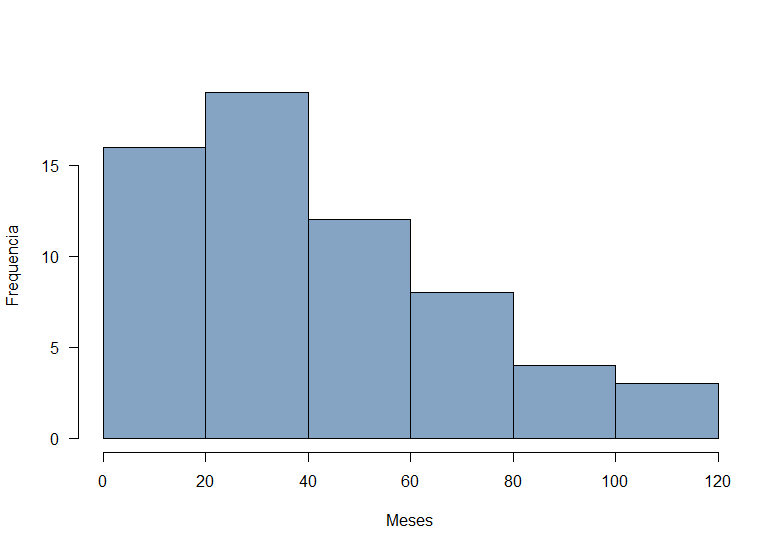
\includegraphics[scale=0.45]{hist.png}
\end{figure}

\hypertarget{muxe9todos}{%
\section*{Métodos}\label{muxe9todos}}
\addcontentsline{toc}{section}{Métodos}

\hypertarget{muxe9todo-de-momentos-casella2021statistical}{%
\subsection{Método de Momentos
(1)}\label{muxe9todo-de-momentos-casella2021statistical}}

El método de momentos para estimar parámetros es considerado uno de los
métodos más viejos y ``confiables''. Es ideal usarlo cuando los
parámetros distribucionales que se quieren estimar están involucrados en
la función de los momentos teóricos (comúnmente en media y varianza
poblacional). El argumento en el que se basa su implementación es muy
intuitivo: usar el principio de analogía muestral, estimando con las
contrapartes muestrales los momentos teóricos, para obtener las
estimaciones de los parámetros distribucionales deseados.

Sea \(X_1, \ldots , X_n\) una muestra aleatoria de una población cuya
función de densidad o masa es
\(f(x \, | \, \theta_1, \ldots , \theta_k)\), donde \(\theta_i\) es el
i-ésimo parámetro de la distribución que se desea estimar. El método de
momentos consiste en igualar los \(k\) momentos teóricos con los \(k\)
momentos muestrales para resolver el sistema de ecuaciones simultáneas
que se genera.

Formalmente definimos:

\begin{equation*}
\begin{aligned}
m_{1} &=\frac{1}{n} \sum_{i=1}^{n} X_{i}^{1}, \quad \mu_{1}=\mathbb{E}[ X^{1}], \\
m_{2} &=\frac{1}{n} \sum_{i=1}^{n} X_{i}^{2}, \quad \mu_{2}=\mathbb{E}[ X^{2}], \\
& \vdots \\
m_{k} &=\frac{1}{n} \sum_{i=1}^{n} X_{i}^{k}, \quad \mu_{k}=\mathbb{E}[ X^{k}] .
\end{aligned}
\end{equation*}

Los momentos teóricos típicamente son una función del vector de
parámetros \((\theta_1, \ldots, \theta_k)\), es decir,
\(\mu_j(\theta_1, \ldots, \theta_k)\). Así pues, el método de momentos
obtiene los estimadores \((\hat{\theta_1}, \ldots, \hat{\theta_k})\)
resolviendo el siguiente sistema de ecuaciones de
\((\theta_1, \ldots, \theta_k)\) en términos de de
\((m_1, \ldots, m_k)\):

\begin{equation*}
    \begin{aligned}
m_{1} &=\mu_{1}\left(\theta_{1}, \ldots, \theta_{k}\right) \\
m_{2} &=\mu_{2}\left(\theta_{1}, \ldots, \theta_{k}\right) \\
& \vdots \\
m_{k} &=\mu_{k}\left(\theta_{1}, \ldots, \theta_{k}\right)
\end{aligned}
\end{equation*}

Existen otras formas más flexibles de implementar el método de momentos,
como el método de momentos generalizado. Por ejemplo, los coeficientes
de un modelo de regresión lineal pueden obtenerse por este método
igualando los momentos teóricos de las ecuaciones normales del problema
de minimización (condiciones de primer orden) con el vector de ceros.
Usando el principio de analogía, igualamos las contrapartes muestrales
de los momentos teóricos con un vector de ceros y resolvemos el sistema
de ecuaciones homogéneo. Asimismo, existen distintas versiones del
método que se pueden utilizar para modelos identificados (mismo número
de ecuaciones que parámetros a estimar) y sobre-identificados (más
ecuaciones que parámetros a estimar).

\hypertarget{muxe9todo-de-newton-ascher2011first}{%
\subsection{Método de Newton
(2)}\label{muxe9todo-de-newton-ascher2011first}}

El método de Newton es uno de los métodos numéricos más básicos que se
pueden utilizar para encontrar las raíces de una función. Supongamos que
nuestra función \(f\) es tal que \(f \in C^2[a,b]\). Sea \(x_k\) una
iteración del método. Recordemos que el teorema de Taylor nos dice que
para \(f \in C^{k+1}[a,b]\) con \(x, \, x_0 \in [a,b]\) y
\(h\in\mathbb{R}\) tenemos que

\begin{equation*}
    \begin{aligned}
        f\left(x_{0}+h\right) &=f\left(x_{0}\right)+h f^{\prime}\left(x_{0}\right)+\frac{h^{2}}{2} f^{\prime \prime}\left(x_{0}\right)+\cdots+\frac{h^{k}}{k !} f^{(k)}\left(x_{0}\right) \\
        &+\frac{h^{k+1}}{(k+1) !} f^{(k+1)}(\xi)
    \end{aligned}
\end{equation*}

donde \(\xi \in(x_0,x_0+h)\).

Así pues, podemos escribir a \(f(x)=f(x+x_k-x_k)\) como sigue

\[
    f(x)=f\left(x_{k}\right)+f^{\prime}\left(x_{k}\right)\left(x-x_{k}\right)+\frac{f^{\prime \prime}(\xi(x))\left(x-x_{k}\right)^{2}}{2} 
\]

donde \(\xi(x)\) es un punto desconocido en el intervalo \((x,x_k)\).

Sea \(x=x^*\) tal que \(f(x^*)=0\). Si \(f\) fuera una función lineal
entonces el problema sería realmente sencillo ya que
\(f^{\prime\prime}\equiv0\), por lo que podríamos encontrar la raíz de
la función resolviendo

\[f\left(x_{k}\right)+f^{\prime}\left(x_{k}\right)\left(x^{*}-x_{k}\right) = 0,\]

dándonos como resultado

\[x^{*}=x_{k}-f\left(x_{k}\right) / f^{\prime}\left(x_{k}\right).\]

Si la función \(f\) no es lineal entonces definimos la siguiente formula
iterativa para \(x_k\):

\[
x_{k+1}=x_{k}-\frac{f\left(x_{k}\right)}{f^{\prime}\left(x_{k}\right)}, \quad k=0,1,2, \ldots
\]

Al definir de esta forma la regla de actualización de la iteración
\(x_k\), ignoramos el factor
\(f^{\prime \prime}\left(\xi\left(x^{*}\right)\right)\left(x^{*}-x_{k}\right)^{2} / 2\)
de la expansión de Taylor que realizamos, ya que si \(x_k\) está cerca
de \(x^*\) entonces la diferencia \(\left(x^{*}-x_{k}\right)\) es muy
pequeña, por lo que podríamos suponer razonablemente que la siguiente
iteración \(x_{k+1}\) está cerca de \(x^*\) aun si no es considere dicho
término.

\hypertarget{estimaciuxf3n-monte-carlo-dobrow2016introduction}{%
\subsection{Estimación Monte Carlo
(3)}\label{estimaciuxf3n-monte-carlo-dobrow2016introduction}}

Dado un evento \(A\), la estimación Monte Carlo de la probabilidad del
evento A \(\mathbb{P}(A)\) se obtiene repitiendo el experimento
aleatorio un número definido de veces y tomar la proporción de intentos
exitosos en los que el evento \(A\) sucede como una aproximación de
\(\mathbb{A}\).

Esta forma de estimación de las probabilidades de eventos aleatorios es
intuitiva y corresponde a la concepción general de cómo deberían
comportarse las probabilidades. La estimación Monte Carlo nos dice que
la probabilidad de un evento es la proporción de largo plazo de que ese
evento suceda repetidas veces en pruebas aleatorizadas.

Este método está justificado formalmente por la Ley Fuerte de los
Grandes Números. Sea \(1_k\) la indicadora de ocurrencia del evento
\(A\) en el \(k\)-ésimo intento, luego

\[\frac{1}{n}\sum_{k=1}^n 1_k\]

es la proporción de que en \(n\) intentos suceda el evento \(A\).
Suponiendo que las \(1_k\) son idénticamente distribuidas tenemos que
\(\mathbb{E}(1_k)=\mathbb{P}(A), \,\, \forall k\).

Luego, por la Ley Fuerte de los Grandes Números

\[\lim_{n\to\infty} \frac{1}{n}\sum_{k=1}^n = \mathbb{P}(A), \text{ con probabilidad 1.}\]

Es decir, para \(n\) grande el estimador Monte Carlo de la probabilidad
del evento \(A\) es

\[\frac{1}{n}\sum_{k=1}^n \approx \mathbb{P}(A) .\]

\hypertarget{algoritmo-para-muxe9todo-de-momentos-con-simulaciuxf3n-monte-carlo}{%
\subsection{Algoritmo para Método de Momentos con Simulación Monte
Carlo}\label{algoritmo-para-muxe9todo-de-momentos-con-simulaciuxf3n-monte-carlo}}

Suponemos que la distribución a estimar sigue una distribución gamma con
parámetros \(\theta = (\alpha, \beta)\), dónde \(\alpha > 0\) es el
parámetro de forma y \(\beta > 0\) es el parámetro de escala, tal que su
función de densidad está dada por:

\[f(x;\theta) = \frac{1}{\Gamma(\alpha)\beta^{\alpha}}x^{\alpha-1}e^{-\frac{x}{\beta}}, \qquad x\in(0,\infty)\]
Sea \(\mu(\theta)\) el vector de momentos teóricos de interés de la
distribución gamma con parámetros \(\theta = (\alpha, \beta)\). En
particular, consideramos la media y la varianza de la distribución
gamma:

\[\mu(\theta) = \begin{bmatrix} \mu \\ \sigma^{2} \end{bmatrix}\]

Sea \(\mu_{0}\) el vector de momentos muestrales de los datos observados
en nuestra base que buscamos reproducir. En nuestro caso, buscamos
reproducir la media y la varianza muestral, tal que:

\[\mu_{0} = \begin{bmatrix} \Bar{x} \\ Var(x) \end{bmatrix}\]

Comenzamos nuestra estimación proponiendo un valor inicial para los
parámetros que caracterizan a la distribución:
\(\theta_{0} = (\alpha_{0}, \beta_{0})\). Después realizamos el
siguiente proceso iterativo por \(t\) iteraciones o hasta que alcancemos
un nivel de tolerancia deseado en los valores estimados de los
parámetros.

Para cada iteración \(t = 1, 2, \dots\):

\begin{enumerate}
    \item Muestreamos $N_{t}$ observaciones de la distribución gamma con parámetros $\theta_{t}$. 
    \item Estimamos $\mu(\theta)$ y $\mu^{\prime}(\theta)$ mediante el uso de estimadores Monte Carlo.
    \item Utilizamos las estimaciones de $\hat{\mu}(\theta)$ y $\hat{\mu}^{\prime}(\theta)$ para obtener $\theta_{t+1}$ mediante el método Newton-Raphson.
    \item Verificamos que $\theta_{t+1}$ sea parte del espacio de parámetros de la distribución gamma ($\theta > 0$), de lo contrario, mantenemos el valor de $\theta_{t}$.
\end{enumerate}

Los estimadores Monte Carlo que utilizamos para estimar \(\mu(\theta)\)
y \(\mu^{\prime}(\theta)\) provienen de los propuestos por Gelman (4).
Dado que \(\mu(\theta) = \mathbb{E}[h(x)|\theta]\), donde \(h(x)\) es
función dada, el estimador Monte Carlo para \(\mu(\theta)\) es:

\[\hat{\mu}(\theta) = \frac{1}{N} \sum_{i = 1}^{N} h(x_{i})\]

Por otro lado,

\begin{align*}
\mu^{\prime}(\theta) &= \frac{d}{d\theta}\mathbb{E}[h(x)|\theta] \\
&= \int h(x) \frac{d}{d\theta} f(x;\theta) dx \\
&= \mathbb{E}[h(x)U(x,\theta)^{T}]
\end{align*}

Donde \(U(x,\theta)^{T} = \frac{d}{d\theta} \log{f(x;\theta)}\). Sea
entonces el estimador Monte Carlo para \(\mu^{\prime}(\theta)\):

\[\hat{\mu}^{\prime}(\theta) = \frac{1}{N} \sum_{i = 1}^{N} h(x_{i})U(x_{i},\theta)^{T}\]

Para la implementación del algoritmo en nuestro caso particular, tomamos
en cuenta lo siguiente. El vector de parámetros a estimar bidimensional,
dado por: \(\theta=(\alpha,\beta)\); la función
\(h(\vec{x})=(x_i, (x_i - \overline{\mathbf{x}})^{2})\) y, finalmente,
nuestro sistema de ecuaciones
\(U(x,\theta)= d / d \theta (log(f(\vec{x})))\), dado por:

\[ \begin{cases} \frac{\displaystyle d}{\displaystyle d\alpha}=-\frac{\displaystyle \Gamma'(\alpha)}{\displaystyle \Gamma(\alpha)}-ln(\beta)+ln(x_i) \\ \frac{\displaystyle d}{\displaystyle d\beta}= -\frac{\displaystyle \alpha}{\displaystyle \beta} + \frac{\displaystyle x_i}{\displaystyle \beta^{2}}  \end{cases} \qquad i=1,2,...,N \]

Después de definir las ecuaciones y funciones necesarias para el
algoritmo, usamos los resultados de las simulaciones de la distribución
objetivo para calcular \(\hat{\mu}^{\prime}(\theta)\),
\(\hat{\mu}(\theta)\) y después, realizar la siguiente iteración del
algoritmo de Newton-Raphson en 2 dimensiones, dada por:

\[ \theta_{t+1} = \theta_t + [\hat{\mu}^{\prime}(\theta_t)]^{-1} \cdot (\mu_0 - \hat{\mu}(\theta_t)) \qquad t=1,2,... \]

donde \(\theta_t\) es un vector de 2x1 que contiene el valor de los
parámetros de la iteración actual, \(\hat{\mu}^{\prime}(\theta_t)\) es
una matriz de 2x2, \(\mu_0\) es un vector que contiene la media y
varianza muestral y \(\hat{\mu}(\theta)\) es un vector de 2x1.

Al implementar el algoritmo propuesto por Gelman, nos encontramos con 2
dificultades principales; la primera, fue que había iteraciones donde el
parámetro \(\alpha\) era menor a 0 y por lo tanto, se encontraba fuera
del espacio paramétrico y el algoritmo no podía concluir. Por lo tanto,
implementamos una condición que solo tomara los valores positivos de los
parámetros y en caso de encontrar uno negativo, quedarse en la
estimación del paso anterior y repetir el algoritmo. De aquí, surgió la
segunda dificultad: al encontrarse con un valor negativo, las
estimaciones aterrizaban en el valor estimado anterior y no cambiaban
durante el resto del algoritmo. Para resolver este problema, cambiamos
la condición a que el algoritmo tomara el valor de la estimación
anterior más un error estocástico distribuido \(Unif(0,1)\) y así,
logramos que el algoritmo evitara valores fuera del espacio paramétrico
y que no se estancara en la estimación anterior en caso de hacerlo.

\hypertarget{resultados}{%
\section*{Resultados}\label{resultados}}
\addcontentsline{toc}{section}{Resultados}

\begin{Shaded}
\begin{Highlighting}[]
\NormalTok{gamma.moments }\OtherTok{\textless{}{-}} \ControlFlowTok{function}\NormalTok{(}
\NormalTok{        data, iters, alpha}\FloatTok{.0}\NormalTok{, beta}\FloatTok{.0}
\NormalTok{) \{}
\NormalTok{  sample.mean }\OtherTok{\textless{}{-}} \FunctionTok{mean}\NormalTok{(data)}
\NormalTok{  sample.var }\OtherTok{\textless{}{-}} \FunctionTok{var}\NormalTok{(data)}
\NormalTok{  mu}\FloatTok{.0} \OtherTok{\textless{}{-}} \FunctionTok{c}\NormalTok{(sample.mean, sample.var)}
\NormalTok{  theta }\OtherTok{\textless{}{-}} \FunctionTok{matrix}\NormalTok{(}\ConstantTok{NA}\NormalTok{, }\DecValTok{2}\NormalTok{, iters)}
\NormalTok{  theta[, }\DecValTok{1}\NormalTok{] }\OtherTok{\textless{}{-}} \FunctionTok{c}\NormalTok{(alpha}\FloatTok{.0}\NormalTok{, beta}\FloatTok{.0}\NormalTok{)}

  \ControlFlowTok{for}\NormalTok{ (i }\ControlFlowTok{in} \DecValTok{2}\SpecialCharTok{:}\NormalTok{iters) \{}
\NormalTok{    n }\OtherTok{\textless{}{-}}\NormalTok{ i }\SpecialCharTok{+} \DecValTok{100}
\NormalTok{    simulated }\OtherTok{\textless{}{-}} \FunctionTok{rgamma}\NormalTok{(}
\NormalTok{            n,}
            \AttributeTok{shape =}\NormalTok{ theta[}\DecValTok{1}\NormalTok{, i }\SpecialCharTok{{-}} \DecValTok{1}\NormalTok{],}
            \AttributeTok{scale =}\NormalTok{ theta[}\DecValTok{2}\NormalTok{, i }\SpecialCharTok{{-}} \DecValTok{1}\NormalTok{]}
\NormalTok{    )}
\NormalTok{    mu }\OtherTok{\textless{}{-}} \FunctionTok{c}\NormalTok{(}\FunctionTok{mean}\NormalTok{(simulated), }\FunctionTok{var}\NormalTok{(simulated))}
\NormalTok{    mu.hat }\OtherTok{\textless{}{-}} \FunctionTok{matrix}\NormalTok{(}\DecValTok{0}\NormalTok{, }\DecValTok{2}\NormalTok{, }\DecValTok{2}\NormalTok{)}
\NormalTok{    h }\OtherTok{\textless{}{-}}\NormalTok{ u }\OtherTok{\textless{}{-}} \ConstantTok{NULL}

    \ControlFlowTok{for}\NormalTok{ (j }\ControlFlowTok{in} \DecValTok{1}\SpecialCharTok{:}\FunctionTok{length}\NormalTok{(simulated)) \{}
\NormalTok{      u[}\DecValTok{1}\NormalTok{] }\OtherTok{\textless{}{-}} \SpecialCharTok{{-}}\FunctionTok{digamma}\NormalTok{(theta[}\DecValTok{1}\NormalTok{, i }\SpecialCharTok{{-}} \DecValTok{1}\NormalTok{]) }\SpecialCharTok{{-}}
              \FunctionTok{log}\NormalTok{(theta[}\DecValTok{2}\NormalTok{, i }\SpecialCharTok{{-}} \DecValTok{1}\NormalTok{]) }\SpecialCharTok{+}
              \FunctionTok{log}\NormalTok{(simulated[j])}
\NormalTok{      u[}\DecValTok{2}\NormalTok{] }\OtherTok{\textless{}{-}}\NormalTok{ (}\SpecialCharTok{{-}}\NormalTok{theta[}\DecValTok{1}\NormalTok{, i }\SpecialCharTok{{-}} \DecValTok{1}\NormalTok{] }\SpecialCharTok{/}\NormalTok{ theta[}\DecValTok{2}\NormalTok{, i }\SpecialCharTok{{-}} \DecValTok{1}\NormalTok{]) }\SpecialCharTok{+}
\NormalTok{              simulated[j] }\SpecialCharTok{/}\NormalTok{ (theta[}\DecValTok{2}\NormalTok{, i }\SpecialCharTok{{-}} \DecValTok{1}\NormalTok{]}\SpecialCharTok{\^{}}\DecValTok{2}\NormalTok{)}
\NormalTok{      h[}\DecValTok{1}\NormalTok{] }\OtherTok{\textless{}{-}}\NormalTok{ simulated[j]}
\NormalTok{      h[}\DecValTok{2}\NormalTok{] }\OtherTok{\textless{}{-}}\NormalTok{ (simulated[j] }\SpecialCharTok{{-}} \FunctionTok{mean}\NormalTok{(simulated))}\SpecialCharTok{\^{}}\DecValTok{2}
\NormalTok{      m }\OtherTok{\textless{}{-}}\NormalTok{ h }\SpecialCharTok{\%*\%} \FunctionTok{t}\NormalTok{(u)}
\NormalTok{      mu.hat }\OtherTok{\textless{}{-}}\NormalTok{ mu.hat }\SpecialCharTok{+}\NormalTok{ m}
\NormalTok{    \}}

\NormalTok{    mu.hat }\OtherTok{\textless{}{-}}\NormalTok{ mu.hat }\SpecialCharTok{/} \FunctionTok{length}\NormalTok{(simulated)}

\NormalTok{    par }\OtherTok{\textless{}{-}}\NormalTok{ theta[, i }\SpecialCharTok{{-}} \DecValTok{1}\NormalTok{] }\SpecialCharTok{+}
            \FunctionTok{solve}\NormalTok{(mu.hat) }\SpecialCharTok{\%*\%}\NormalTok{ (mu}\FloatTok{.0} \SpecialCharTok{{-}}\NormalTok{ mu)}

    \ControlFlowTok{if}\NormalTok{ (par[}\DecValTok{1}\NormalTok{] }\SpecialCharTok{*}\NormalTok{ par[}\DecValTok{2}\NormalTok{] }\SpecialCharTok{\textgreater{}} \DecValTok{0}\NormalTok{) \{}
\NormalTok{      theta[, i] }\OtherTok{\textless{}{-}}\NormalTok{ par}
\NormalTok{    \} }\ControlFlowTok{else}\NormalTok{ \{}
\NormalTok{      theta[, i] }\OtherTok{\textless{}{-}}\NormalTok{ theta[, i }\SpecialCharTok{{-}} \DecValTok{1}\NormalTok{] }\SpecialCharTok{+}
              \FunctionTok{runif}\NormalTok{(}\DecValTok{1}\NormalTok{)}
\NormalTok{    \}}
\NormalTok{  \}}

\NormalTok{  theta }\OtherTok{\textless{}{-}} \FunctionTok{data.frame}\NormalTok{(}
          \AttributeTok{x =}\NormalTok{ theta[}\DecValTok{1}\NormalTok{,],}
          \AttributeTok{y =}\NormalTok{ theta[}\DecValTok{2}\NormalTok{,],}
          \AttributeTok{n =} \DecValTok{1}\SpecialCharTok{:}\NormalTok{iters}
\NormalTok{  )}

\NormalTok{  p}\FloatTok{.1} \OtherTok{\textless{}{-}} \FunctionTok{ggplot}\NormalTok{(theta) }\SpecialCharTok{+}
    \FunctionTok{geom\_line}\NormalTok{(}\FunctionTok{aes}\NormalTok{(}\AttributeTok{x =}\NormalTok{ n, }\AttributeTok{y =}\NormalTok{ x),}
              \AttributeTok{size =} \FloatTok{0.1}\NormalTok{) }\SpecialCharTok{+}
    \FunctionTok{labs}\NormalTok{(}\AttributeTok{title =} \ConstantTok{NULL}\NormalTok{,}
         \AttributeTok{x =} \StringTok{"n"}\NormalTok{,}
         \AttributeTok{y =} \FunctionTok{expression}\NormalTok{(alpha),}
         \AttributeTok{caption =} \FunctionTok{paste}\NormalTok{(}\StringTok{"alpha inicial ="}\NormalTok{,}
\NormalTok{                         alpha}\FloatTok{.0}\NormalTok{,}
                         \StringTok{"}\SpecialCharTok{\textbackslash{}n}\StringTok{beta inicial ="}\NormalTok{,}
\NormalTok{                         beta}\FloatTok{.0}\NormalTok{))}

\NormalTok{  p}\FloatTok{.2} \OtherTok{\textless{}{-}} \FunctionTok{ggplot}\NormalTok{(theta) }\SpecialCharTok{+}
    \FunctionTok{geom\_line}\NormalTok{(}\FunctionTok{aes}\NormalTok{(}\AttributeTok{x =}\NormalTok{ n, }\AttributeTok{y =}\NormalTok{ y),}
              \AttributeTok{size =} \FloatTok{0.1}\NormalTok{) }\SpecialCharTok{+}
    \FunctionTok{labs}\NormalTok{(}\AttributeTok{title =} \ConstantTok{NULL}\NormalTok{,}
         \AttributeTok{x =} \StringTok{"n"}\NormalTok{,}
         \AttributeTok{y =} \FunctionTok{expression}\NormalTok{(beta),}
         \AttributeTok{caption =} \FunctionTok{paste}\NormalTok{(}\StringTok{"alpha inicial ="}\NormalTok{,}
\NormalTok{                         alpha}\FloatTok{.0}\NormalTok{,}
                         \StringTok{"}\SpecialCharTok{\textbackslash{}n}\StringTok{beta inicial ="}\NormalTok{,}
\NormalTok{                         beta}\FloatTok{.0}\NormalTok{))}

\NormalTok{  shape }\OtherTok{\textless{}{-}} \FunctionTok{mean}\NormalTok{(theta}\SpecialCharTok{$}\NormalTok{x)}
\NormalTok{  scale }\OtherTok{\textless{}{-}} \FunctionTok{mean}\NormalTok{(theta}\SpecialCharTok{$}\NormalTok{y)}

\NormalTok{  dist.mean }\OtherTok{\textless{}{-}} \FunctionTok{mean}\NormalTok{(shape }\SpecialCharTok{*}\NormalTok{ scale)}
\NormalTok{  dist.var }\OtherTok{\textless{}{-}} \FunctionTok{mean}\NormalTok{(shape }\SpecialCharTok{*}\NormalTok{ (scale}\SpecialCharTok{\^{}}\DecValTok{2}\NormalTok{))}

\NormalTok{  test }\OtherTok{\textless{}{-}} \FunctionTok{ks.test}\NormalTok{(}
\NormalTok{          data, }\StringTok{"pgamma"}\NormalTok{,}
          \AttributeTok{shape =}\NormalTok{ shape, }\AttributeTok{scale =}\NormalTok{ scale}
\NormalTok{  )}

\NormalTok{  results }\OtherTok{\textless{}{-}} \FunctionTok{list}\NormalTok{(}
\NormalTok{          test,}
\NormalTok{          p}\FloatTok{.1}\NormalTok{, p}\FloatTok{.2}\NormalTok{,}
\NormalTok{          shape, scale,}
\NormalTok{          dist.mean, dist.var,}
\NormalTok{          sample.mean, sample.var}
\NormalTok{  )}

  \FunctionTok{return}\NormalTok{(results)}
\NormalTok{\}}
\end{Highlighting}
\end{Shaded}

Para nuestras simulaciones, usamos 1000 iteraciones y distintos valores
iniciales para estimar \(\alpha\) y \(\beta\). Esto es relevante porque
el algoritmo es sensible a la cercanía del valor inicial respecto al
valor de convergencia como podemos observar en las siguientes tabla y
gráficas.

\begin{table}[htbp]
\centering
\begin{tabular}{rrrr}
&       &       &  \\
\midrule
\midrule
\multicolumn{4}{c}{Tabla de resultados para distintos valores iniciales} \\
\multicolumn{1}{c}{$(\alpha_0, \beta_0)$} & \multicolumn{1}{c}{(0.01,  0.01)} & \multicolumn{1}{c}{(2.5, 16.5)} & \multicolumn{1}{c}{(20, 50)} \\
\midrule
\multicolumn{1}{c}{$\alpha$} & \multicolumn{1}{c}{2.4986} & \multicolumn{1}{c}{2.476} & \multicolumn{1}{c}{2.6199} \\
\multicolumn{1}{c}{$\beta$} & \multicolumn{1}{c}{16.6873} & \multicolumn{1}{c}{16.6989} & \multicolumn{1}{c}{16.6827} \\
\multicolumn{1}{c}{$\hat{\mu}$} & \multicolumn{1}{c}{41.6944} & \multicolumn{1}{c}{41.3465} & \multicolumn{1}{c}{43.7063} \\
\multicolumn{1}{c}{$\hat{\sigma}^2$} & \multicolumn{1}{c}{695.7655} & \multicolumn{1}{c}{690.4403} & \multicolumn{1}{c}{729.1397} \\
\multicolumn{1}{c}{$\bar{X}$} & \multicolumn{1}{c}{41.7742} & \multicolumn{1}{c}{41.7742} & \multicolumn{1}{c}{41.7742} \\
\multicolumn{1}{c}{$s^2$} & \multicolumn{1}{c}{691.0629} & \multicolumn{1}{c}{691.0629} & \multicolumn{1}{c}{691.0629} \\
\midrule
\midrule
&       &       &  \\
\end{tabular}%
\label{tab:addlabel}%
\end{table}

\%

\begin{flushleft}\includegraphics{/home/carlos/Documents/simulation-fall-2021/term-paper/term-paper_files/figure-latex/plots-1} \end{flushleft}

\begin{flushleft}\includegraphics{/home/carlos/Documents/simulation-fall-2021/term-paper/term-paper_files/figure-latex/plots-2} \end{flushleft}

\begin{verbatim}
## 
##  One-sample Kolmogorov-Smirnov test
## 
## data:  data
## D = 0.092, p-value = 0.7
## alternative hypothesis: two-sided
\end{verbatim}

\begin{flushleft}\includegraphics{/home/carlos/Documents/simulation-fall-2021/term-paper/term-paper_files/figure-latex/plots-3} \end{flushleft}

\begin{flushleft}\includegraphics{/home/carlos/Documents/simulation-fall-2021/term-paper/term-paper_files/figure-latex/plots-4} \end{flushleft}

\begin{verbatim}
## 
##  One-sample Kolmogorov-Smirnov test
## 
## data:  data
## D = 0.087, p-value = 0.7
## alternative hypothesis: two-sided
\end{verbatim}

\begin{flushleft}\includegraphics{/home/carlos/Documents/simulation-fall-2021/term-paper/term-paper_files/figure-latex/plots-5} \end{flushleft}

\begin{flushleft}\includegraphics{/home/carlos/Documents/simulation-fall-2021/term-paper/term-paper_files/figure-latex/plots-6} \end{flushleft}

\begin{verbatim}
## 
##  One-sample Kolmogorov-Smirnov test
## 
## data:  data
## D = 0.12, p-value = 0.3
## alternative hypothesis: two-sided
\end{verbatim}

\hypertarget{conclusiones}{%
\section*{Conclusiones}\label{conclusiones}}
\addcontentsline{toc}{section}{Conclusiones}

De la aplicación del algoritmo, derivamos múltiples resultados útiles
para el problema que se nos propuso y también recopilamos un conjunto de
limitaciones y alcances que el algoritmo y el trasfondo teórico puede
brindar. A continuación mencionaremos qué podemos inferir de dichos
resultados, el por qué de las limitaciones que enfrentamos y el
desarrollo matemático necesario para ampliar los alcances del estudio.

Los resultados, como se presentaron en la sección anterior, son válidos
y nuestro estudio nos permitirá hacer inferencia sobre los meses que
tarda en regresar el cáncer a los pacientes de cáncer de colon. La
prueba de bondad y ajuste (Kolmogorov-Smirnoff) que realizamos sobre la
muestra y los parámetros teóricos que se estimaron con el algoritmo
indican que existe evidencia estadística suficiente para asumir que la
muestra proviene de una distribución Gamma con los parámetros estimados.
A partir de este resultado, podemos hacer inferencia sobre la variable
aleatoria estudiada y determinar, por ejemplo, el tiempo esperado en el
cual los pacientes volverán a presentar síntomas y la probabilidad de
que regrese el tumor en cierto tiempo.

Las dificultades principales que enfrentamos al implementar el algoritmo
fueron, como se mencionó en el apartado anterior, estimaciones fuera del
espacio paramétrico y el estancamiento del algoritmo en un estado. Como
se comentó, se agregaron condiciones sobre los parámetros para que
fueran únicamente positivos y en caso de estimar un valor negativo, el
algoritmo permanece en el estado anterior más una perturbación
estocástica uniforme entre 0 y 1.

Un aspecto importante dentro de la implementación del algoritmo es la
velocidad de convergencia del mismo. Al emplear métodos como
Newton-Raphson multidimensional y simulación Monte Carlo para estimar
los momentos, es evidente que el algoritmo tendrá cierta velocidad de
convergencia. En el trabajo publicado por Gelman se menciona que, al
momento de simular las observaciones de la distribución teórica, la
velocidad del algoritmo depende de lo siguiente: conforme aumente el
valor del paso \(t\) del algoritmo de Newton-Raphson, para garantizar
convergencia también habrá que aumentar el tamaño de la muestra
simulada. Y, en efecto, nuestro primer intento con un tamaño de muestra
fijo no se mantenía en un valor exacto y, al actualizar el modelo y
aumentar el tamaño de muestra en cada iteración, el algoritmo sí
convergió a un valor. También, como se menciona en el artículo, este
detalle hace que el algoritmo sea ineficiente, ya que hay que simular
una nueva muestra de tamaño creciente en cada iteración.

Para hacer más eficiente el algoritmo, el autor propone hacer muestro
por importancia y de esta forma hacer las iteraciones del algoritmo de
Newton-Raphson con un conjunto fijo de valores simulados. De esta forma,
se pueden hacer \(n\) pasos del algoritmo de Newton-Raphson son solo una
simulación y después de cierto tiempo, volver a simular una muestra y
así acelerar el proceso.

Los alcances que tiene el proyecto son vastos y también mencionados en
el trabajo de Gelman. En primer lugar y, evidentemente, el algoritmo es
una herramienta con un gran trasfondo matemático y estadístico, por lo
cual se puede trabajar con distribuciones de las cuales no conocemos la
constante normalizadora. En nuestro caso, se empleó una distribución
conocida y simple, para evidenciar que el algoritmo funciona a escala
pequeña. Sin embargo, se puede extender, como se mencionó, a
distribuciones cuya constante normalizadora sea una expresión difícil de
calcular. También, como se menciona en el párrafo anterior, se puede
emplear muestreo por importancia para hacer el algoritmo más eficiente.
Otra alternativa para la cual se puede ajustar el algoritmo es, como se
revisó en el curso, en caso de conocer únicamente la distribución
límite, se puede simular la muestra usando el algoritmo de
Metrópolis-Hastings. Finalmente, igual es posible implementar un ajuste
de mínimos cuadrados en el caso de que el problema tenga más momentos
definidos que parámetros (sobredeterminación), y, de esta forma,
implementar el algoritmo de Newton-Raphson con un ajuste de regresión
sobre las ecuaciones normales del problema.

Como pudimos observar, el algoritmo produce resultados y conclusiones
válidas y aplicables en problemas de la vida real e, igualmente, es un
método flexible que puede ajustarse a las múltiples condiciones que
puede presentar cualquier problema. También, descansa sobre múltiples
temas que se revisaron a lo largo del curso y esto permitió mejorar
nuestro entendimiento de qué había que hacer al momento de la
implementación.

\hypertarget{referencias}{%
\section*{Referencias}\label{referencias}}
\addcontentsline{toc}{section}{Referencias}

\showmatmethods
\showacknow
\pnasbreak

\hypertarget{refs}{}
\begin{CSLReferences}{0}{0}
\leavevmode\vadjust pre{\hypertarget{ref-casella2021statistical}{}}%
\CSLLeftMargin{1. }
\CSLRightInline{Casella G, Berger RL (2021) \emph{Statistical inference}
(Cengage Learning).}

\leavevmode\vadjust pre{\hypertarget{ref-ascher2011first}{}}%
\CSLLeftMargin{2. }
\CSLRightInline{Ascher UM, Greif C (2011) \emph{A first course on
numerical methods} (SIAM).}

\leavevmode\vadjust pre{\hypertarget{ref-dobrow2016introduction}{}}%
\CSLLeftMargin{3. }
\CSLRightInline{Dobrow RP (2016) \emph{Introduction to stochastic
processes with r} (John Wiley \& Sons).}

\leavevmode\vadjust pre{\hypertarget{ref-mainArt}{}}%
\CSLLeftMargin{4. }
\CSLRightInline{Gelman A (1995)
\href{http://www.jstor.org/stable/1390626}{Method of moments using monte
carlo simulation}. \emph{Journal of Computational and Graphical
Statistics} 4(1):36--54.}

\end{CSLReferences}



% Bibliography
% \bibliography{pnas-sample}

\end{document}
